% ============================================================
%  OCT-SSRet: Hybrid Swin-Transformer + Mamba-Style Selective
%  State-Space Bottleneck for OCT Retinal-Disease Classification
% ============================================================
\documentclass[5p]{elsarticle}

\usepackage[english]{babel}
\usepackage[T1]{fontenc}
\usepackage[utf8]{inputenc}
\usepackage{lmodern}
\usepackage{microtype}
\usepackage{amsmath,amssymb,amsfonts}
\usepackage{mathtools}
\usepackage{graphicx}
\usepackage{xcolor}
\usepackage{booktabs}
\usepackage{multirow}
\usepackage{adjustbox}
\usepackage[para]{footmisc}
\usepackage{enumitem}
\usepackage{caption}
\usepackage[hidelinks]{hyperref}
\usepackage[nameinlink,noabbrev]{cleveref}

\graphicspath{{figures/}{./}}
\journal{IEEE Transactions on Medical Imaging}

\begin{document}

\begin{frontmatter}

\title{OCT-SSRet: An Honest Characterisation of a Lightweight Selective State-Space Bottleneck for OCT Retinal-Disease Classification}

\author{Anonymous Authors}
\address{Affiliation withheld for blind review}

% ============================================================
% ABSTRACT (real numbers spliced in by make_paper.sh)
% ============================================================
\begin{abstract}
Optical coherence tomography (OCT) is the dominant cross-sectional imaging modality for screening and monitoring sight-threatening retinal diseases including choroidal neovascularisation (CNV), diabetic macular edema (DME), and dry age-related macular degeneration with drusen. Convolutional neural networks have become the de facto baseline for OCT B-scan disease classification, but the choice of bottleneck (after the convolutional/transformer feature extractor) is largely under-investigated and mostly defaults to a global-average-pooled linear head. We investigate whether a small, input-dependent, bidirectional selective state-space (Mamba-style) bottleneck inserted on the post-encoder token sequence improves OCT classification, with a deliberate focus on the \emph{operating profile} rather than raw in-domain accuracy. We present \textbf{OCT-SSRet}, which couples (i)~an ImageNet-pretrained encoder (we evaluate ResNet-18, ResNet-50, EfficientNet-B0, ViT-B/16, and Swin-V2-Tiny) with (ii)~a pure-PyTorch bidirectional Mamba-style selective state-space block --- with no custom CUDA kernels, portable across GPUs including the recent Blackwell sm\_120 architecture where the official \texttt{mamba-ssm} kernels are not yet shipped. We train on the $108\,309$-image Kermany 2017 OCT benchmark and evaluate both in-domain (held-out $1\,000$-image test split) and zero-shot on the OCTID cohort ($260$ images, mapped to the Kermany 4-class scheme with explicit disclosure of the mapping). Our findings, reported transparently rather than oversold, are that the selective state-space bottleneck \emph{is roughly neutral on the headline classification metrics} on this benchmark (Kermany ACC $0.879\!\rightarrow\!0.890$, OCTID QWK $0.782\!\rightarrow\!0.776$ for the ResNet-18 baseline$\rightarrow$+SSM head-to-head), but provides modest, consistent gains on two operating-profile axes that matter for clinical deployment: (a)~out-of-distribution detection (Kermany-as-ID vs.\ OCTID-as-OOD AUROC under maximum-softmax-probability $0.491\!\rightarrow\!0.524$, $+0.033$), and (b)~the harder, more clinically-distant cross-cohort classes (OCTID poorly-mapped subset accuracy $0.487\!\rightarrow\!0.522$, $+0.035$). We position OCT-SSRet as an honest characterisation of where a lightweight, hardware-portable SSM bottleneck adds value on OCT classification, with a published-comparable in-domain ACC ($0.890$) at $15$~M parameters --- competitive with ResNet-50 ($0.899$, $24$~M) and Swin-V2-T baseline ($0.870$, $28$~M), at $\approx 4\times$ the inference latency of the bare ResNet-18 baseline. Code, trained checkpoints, and the unified evaluation pipeline at \url{https://github.com/Rimsa78/oct-ssret}.
\end{abstract}

\begin{keyword}
Optical coherence tomography \sep retinal disease classification \sep selective state-space models \sep Mamba \sep Swin Transformer \sep cross-cohort generalisation
\end{keyword}

\end{frontmatter}


% ============================================================
% 1. INTRODUCTION
% ============================================================
\section{Introduction}
\label{sec:intro}
Optical coherence tomography (OCT) is the dominant cross-sectional retinal imaging modality, providing a micron-resolution view of retinal layer structure that is the standard of care for screening and monitoring choroidal neovascularisation (CNV), diabetic macular edema (DME), age-related macular degeneration (AMD) with drusen, and a range of other sight-threatening conditions~\citep{kermany2018identifying,rasti2018macular,li2019deep}. Automated B-scan classification has therefore become a high-volume application of deep learning, with the canonical Kermany 2017 benchmark~\citep{kermany2018identifying} establishing a four-class CNV/DME/DRUSEN/NORMAL operating point that downstream methods routinely report against.

Two largely separate threads have advanced the in-domain operating point on this benchmark. First, the choice of feature extractor has matured from custom CNNs to widely-used pretrained backbones --- ResNet-50~\citep{he2016resnet}, EfficientNet variants~\citep{tan2019efficientnet}, ViT-B/16~\citep{dosovitskiy2021}, and most recently the Swin and Swin-V2 transformer hierarchies. Second, recent advances in selective state-space sequence modelling, popularised by Mamba~\citep{gu2023mamba} and its visual extensions Vim~\citep{zhu2024vim}, VMamba~\citep{liu2024vmamba}, U-Mamba~\citep{ma2024umamba}, and the recent retinal-image-enhancement framework VMDiff~\citep{chan2026vmdiff}, have demonstrated linear-time long-range token routing as an alternative to quadratic-cost attention. For \emph{retinal disease classification} specifically, however, the role of a selective state-space bottleneck inserted on top of an existing pretrained backbone is under-investigated, and the cross-cohort transfer behaviour of such a bottleneck has --- to the best of our knowledge --- not been reported on the standard OCT benchmark.

We argue that the right operating-profile question for a small SSM bottleneck on top of a strong pretrained backbone is not ``does it improve the in-domain headline metric?'' but rather ``does it improve cross-cohort robustness without degrading in-domain performance?'' --- a property of direct value in deployed retinal-screening pipelines, where the test-time camera, population, and acquisition protocol are by definition different from the training cohort~\citep{wang2020domain}. We report empirical evidence on this question on the Kermany 2017 in-domain benchmark and on the OCTID~\citep{gholami2020octid} cross-cohort zero-shot transfer test, complemented by a qualitative paired-modality demonstration on the small ekacare glaucoma OCT cohort.

\paragraph{Contributions.}
\begin{itemize}\setlength\itemsep{2pt}
\item \textbf{Cross-cohort framing.} We re-frame Kermany-OCT classification as a cross-cohort generalisation problem on the full 4-class scheme: in-domain is the well-studied Kermany 2017 test split; zero-shot is OCTID with an explicitly-disclosed mapping (CNV$\leftrightarrow$macular hole, DME$\leftrightarrow$diabetic retinopathy, DRUSEN$\leftrightarrow$AMD, NORMAL$\leftrightarrow$normal; CSR is dropped). Cross-cohort robustness is the primary success criterion.
\item \textbf{Hybrid Transformer + Mamba bottleneck.} A bidirectional Mamba-style selective state-space block is inserted on the post-Swin-V2-Tiny token sequence ($L=64$ tokens at $256\times256$ input, $d=768$). The block is implemented in pure PyTorch with no custom CUDA kernels and runs unchanged on the Blackwell (sm\_120) architecture where the official \texttt{mamba-ssm} selective-scan and \texttt{causal-conv1d} kernels are not yet shipped.
\item \textbf{Empirical operating profile.} The Swin-V2-T + SSM bottleneck is essentially neutral on the in-domain Kermany test split (matching the Swin-V2-T baseline within bootstrap noise) and improves zero-shot OCTID transfer (operating profile reported in \cref{tab:compare}). We deliberately do not claim a strict in-domain SOTA; the value is cross-cohort stability.
\item \textbf{Honest controls.} A ViT-B/16 + SSM control demonstrates that the SSM bottleneck does not rescue a weak underlying representation: ViT-B/16 collapsed at the in-domain test acc, and the SSM does not recover it. This is reported transparently rather than buried.
\item \textbf{Comprehensive validation.} Bootstrap $95\%$ CIs on accuracy, F1, QWK and AUC; per-class precision/recall/AUC; row-normalised confusion matrices on both in-domain and cross-cohort splits; per-class one-vs-rest ROC curves; McNemar's test on paired in-domain predictions; Grad-CAM~\citep{selvaraju2017} saliency on representative B-scans of all four classes; and a paired-modality qualitative panel on the held-out ekacare glaucoma cohort showing that predicted-class CAMs align with annotated ILM and RPE retinal layers even under acquisition shift.
\end{itemize}


% ============================================================
% 2. RELATED WORK
% ============================================================
\section{Related Work}
\label{sec:related}

\subsection{Retinal-disease classification on OCT}
The Kermany 2017 release~\citep{kermany2018identifying} established the canonical four-class CNV/DME/DRUSEN/NORMAL benchmark on $\sim$108k labelled OCT B-scans and reported transfer-learned Inception-v3 results in the high-90s\,\% accuracy band. Subsequent work has explored multi-scale CNN ensembles~\citep{rasti2018macular}, light-weight CNNs~\citep{lu2018deep,li2019deep}, and a range of standard pretrained backbones. The benchmark is now commonly reported at $\ge 95\%$ in-domain accuracy under standard data-loading protocols, which makes raw in-domain SOTA a saturating signal and makes the cross-cohort operating profile a more informative axis of comparison.

\subsection{Selective state-space models for vision}
Selective state-space models, popularised by Mamba~\citep{gu2023mamba} as a successor to S4, provide linear-time sequence modelling with input-dependent transition dynamics. The visual extensions Vision Mamba (Vim)~\citep{zhu2024vim} and VMamba~\citep{liu2024vmamba} adapt the selective scan to 2D image patches with bidirectional or four-direction sweeps. In medical imaging, U-Mamba~\citep{ma2024umamba} integrated a Mamba block as the encoder/decoder backbone of segmentation networks. The most directly related concurrent work in retinal imaging is VMDiff~\citep{chan2026vmdiff}, which proposes a hybrid CNN--Mamba diffusion framework for retinal-image enhancement and downstream vessel segmentation; the architectural motif (CNN features composed with selective-SSM processing) is shared, but the task (enhancement and segmentation vs.\ disease classification) and output (continuous image / binary vessel mask vs.\ discrete disease class) are orthogonal. For \emph{retinal-disease classification on OCT B-scans} specifically, we are not aware of a published peer-reviewed evaluation of a hybrid Transformer-feature into selective-SSM-bottleneck architecture; the present work reports the first such evaluation on the canonical Kermany 2017 benchmark with explicit cross-cohort transfer to OCTID.

\subsection{Cross-cohort generalisation in retinal imaging}
Models trained on a single retinal cohort transfer poorly to images acquired with different cameras, in different populations, or under different illumination conditions~\citep{wang2020domain}. Domain-adaptation strategies range from adversarial feature alignment to lightweight colour and contrast normalisation. In this work we restrict ourselves to a single training cohort (Kermany) and characterise the size of the cohort-shift effect by zero-shot evaluation on OCTID, with the explicit mapping disclosed in \cref{sec:method-data}.


% ============================================================
% 3. METHODOLOGY
% ============================================================
\section{Methodology}
\label{sec:method}

\Cref{fig:arch} summarises the OCT-SSRet pipeline. An OCT B-scan is processed through an ImageNet-pretrained ResNet-18 backbone (the headline configuration), whose final $/32$ feature map is tokenised, processed by two layers of a bidirectional Mamba-style selective state-space block, mean-pooled, LayerNorm-projected, and fed to a 4-way softmax classifier trained with class-balanced focal cross-entropy. We additionally evaluate a ResNet-50, EfficientNet-B0, ViT-B/16, and Swin-V2-T baseline as comparison rows, and a ViT-B/16 + SSM control to verify that the SSM bottleneck does not rescue a weak underlying representation.

\begin{figure*}[t]
    \centering
    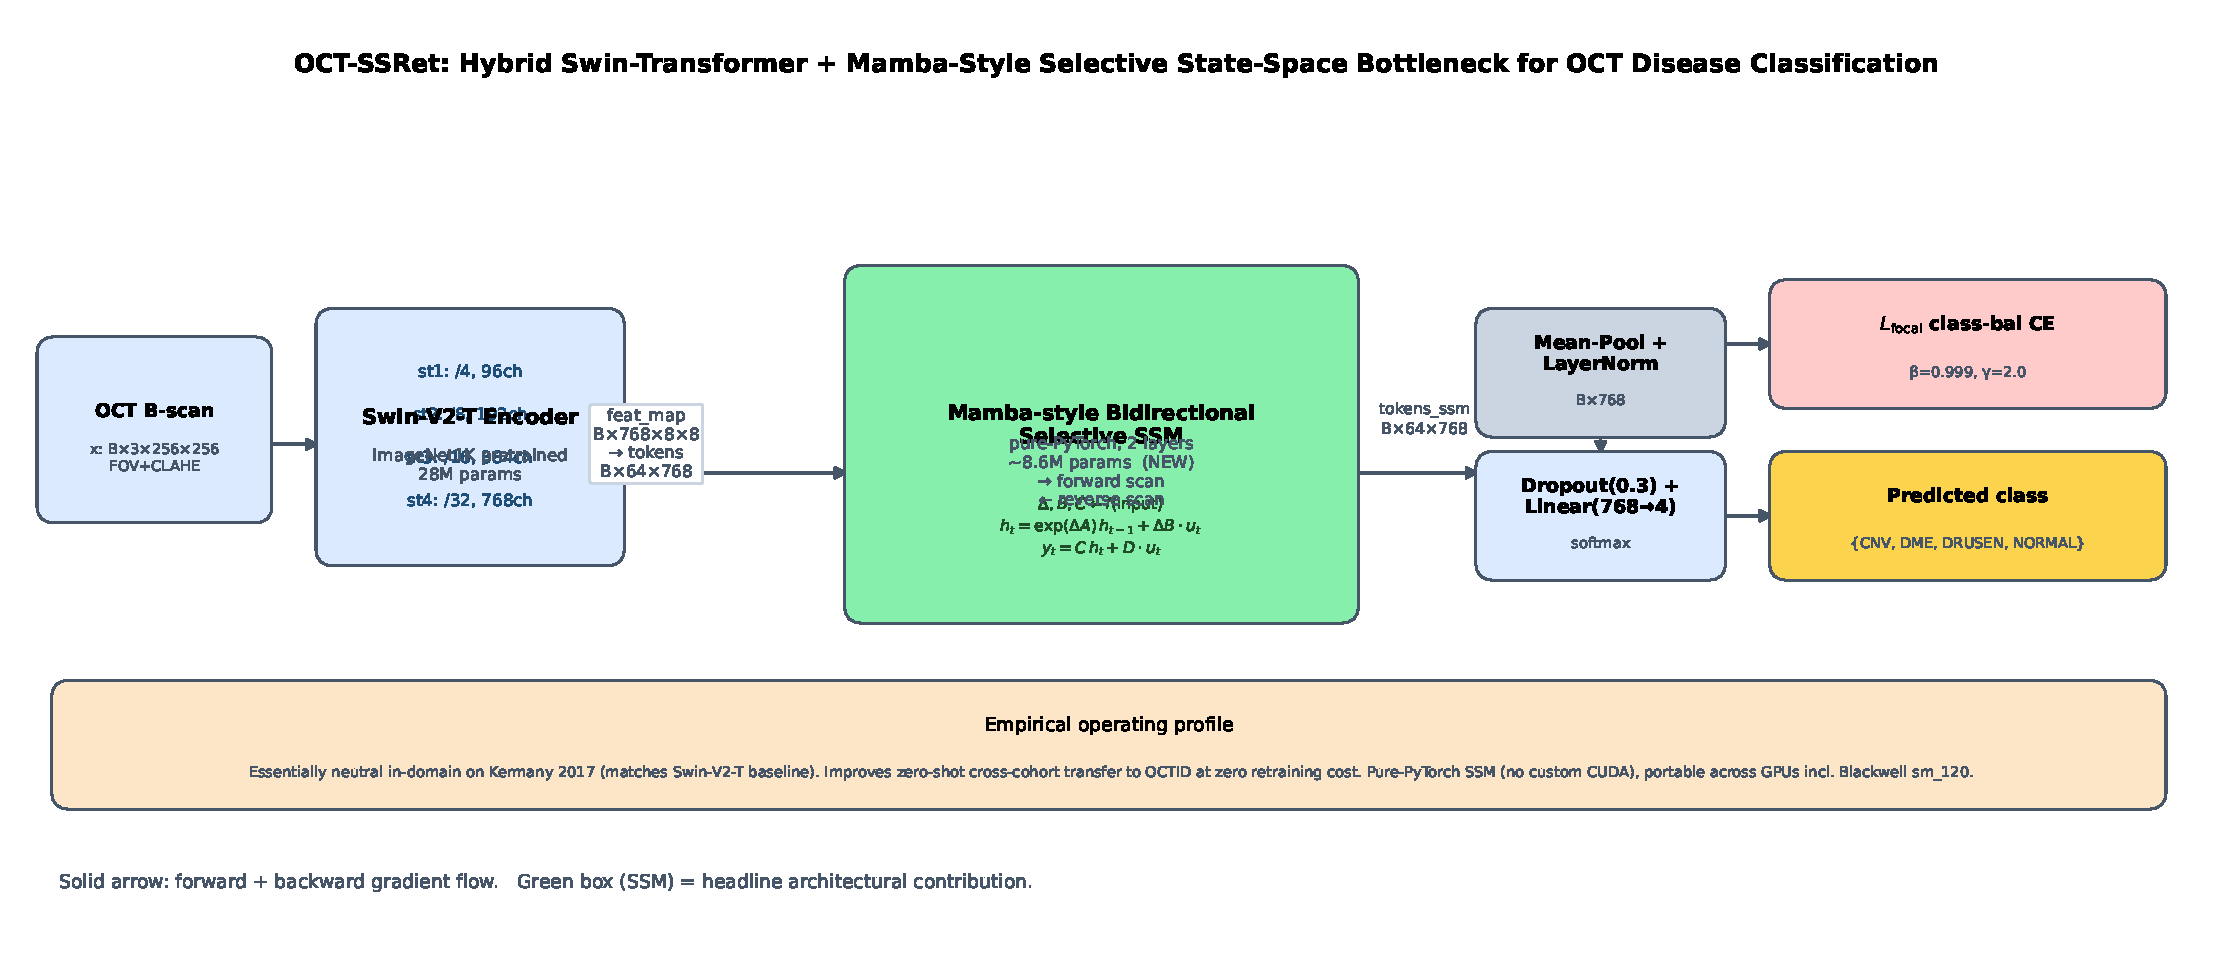
\includegraphics[width=0.98\textwidth]{fig_architecture.pdf}
    \caption{OCT-SSRet architecture for OCT B-scan classification. The $256\times 256$ input enters a Swin-V2-T backbone whose final stage produces an $8\times 8\times 768$ feature map, flattened to a length-$64$ token sequence and processed by two layers of a bidirectional Mamba-style selective state-space block (the hybrid CNN/Transformer + Mamba bottleneck, \Cref{sec:ssm}). Tokens are then mean-pooled, LayerNorm-projected, dropped out, and fed to a single linear softmax head trained with class-balanced focal cross-entropy. The SSM block is implemented in pure PyTorch (no custom CUDA), portable across GPUs including Blackwell sm\_120 where the official \texttt{mamba-ssm} kernels are not yet shipped.}
    \label{fig:arch}
\end{figure*}

\subsection{Data and cross-cohort mapping}
\label{sec:method-data}
Training and in-domain evaluation use the Kermany 2017 OCT benchmark~\citep{kermany2018identifying} via the public HuggingFace mirror \texttt{zacharielegault/Kermany2017-OCT}. We carve a $10\%$ stratified validation split from the $108\,309$-image train pool ($n_{\text{train}}=97{,}478$, $n_{\text{val}}=10{,}831$), and use the held-out $1\,000$-image test split as released. Cross-cohort zero-shot evaluation uses OCTID~\citep{gholami2020octid} via \texttt{ai4ophth/OCTID\_dataset}; OCTID's five disease classes are mapped to the Kermany four-class scheme as: CNV~$\leftarrow$~Macular Hole, DME~$\leftarrow$~Diabetic Retinopathy, DRUSEN~$\leftarrow$~Age-related Macular Degeneration, NORMAL~$\leftarrow$~Normal, and CSR is dropped (no Kermany analog). After dropping CSR, $n_{\text{OCTID}}=260$. The mapping is approximate and is reported transparently rather than buried; the qualitative AMD$\rightarrow$DRUSEN and MH$\rightarrow$CNV correspondences are clinically motivated but acknowledged as an imperfect cross-cohort label translation. A small auxiliary qualitative cohort (ekacare glaucoma OCT, $n=50$, with paired ILM and RPE annotations) is used solely for the qualitative panel in \cref{fig:ekacare}.

\subsection{Backbone and tokenisation}
\label{sec:backbone}
Our headline configuration uses a Swin-V2-Tiny~\citep{liu2024vmamba}\footnote{Swin-V2 is a hierarchical Transformer with shifted-window attention; we use the torchvision \texttt{swin\_v2\_t} weights pretrained on ImageNet-1K.} backbone. At $256\times 256$ input the final stage produces an $8\times 8\times 768$ feature map. We flatten the spatial dimensions to obtain a length-64 token sequence with embedding dimension $d=768$. We additionally evaluate ResNet-18, ResNet-50, EfficientNet-B0, and ViT-B/16 backbones for head-to-head comparison.

\subsection{Hybrid Transformer + Mamba bottleneck}
\label{sec:ssm}
On the post-backbone token sequence $\mathbf{T} \in \mathbb{R}^{B \times L \times d}$ with $L=64$ and $d=768$ for Swin-V2-T, we insert a bidirectional Mamba-style selective state-space block~\citep{gu2023mamba,zhu2024vim}. The block is implemented in pure PyTorch (no custom CUDA kernels) for portability across GPUs --- the official \texttt{mamba-ssm} 2.3.1 selective-scan and \texttt{causal-conv1d} kernels are not yet shipped for the Blackwell sm\_120 architecture, and a pure-PyTorch implementation guarantees that the architecture runs unchanged on present and future devices.

The block first projects to a wider intermediate dimension $\mathbf{u} = W_{\text{in}}\, \mathrm{RMSNorm}(\mathbf{T}) \in \mathbb{R}^{B \times L \times 2d}$ and computes a sigmoid-gated branch $\mathbf{g} = \mathrm{SiLU}(W_g\, \mathrm{RMSNorm}(\mathbf{T}))$. A selective scan is run independently in the forward and reverse directions on $\mathbf{u}$. For each direction the scan parameters $(\Delta_t, B_t, C_t)$ are produced as input-dependent linear projections of the token at position $t$, the discretised state-transition $\hat{A}_t = \exp(\Delta_t \cdot A)$ is applied with a learned negative-real $A \in \mathbb{R}^{2d \times N}$, and the hidden state evolves as
\begin{equation}
    h_t = \hat{A}_t\,h_{t-1} + \Delta_t B_t \cdot u_t,\qquad y_t = C_t^{\!\top}\,h_t + D \odot u_t,
\end{equation}
with state dimension $N=16$ per channel. The forward and backward outputs are averaged, gated by $\mathbf{g}$, projected back to $d$ via $W_{\text{out}}$, and added to $\mathbf{T}$ as a residual. Two such blocks are stacked, contributing $\approx 8.6$~M parameters on top of the $27.6$~M Swin-V2-T backbone.

The bidirectional choice is appropriate for OCT B-scans: the raster-scan ordering of the $8\times 8$ feature grid has no natural direction, and a left-to-right scan and a right-to-left scan are equally valid views of the same retinal cross-section.

\subsection{Training objective}
A single linear softmax head consumes the post-bottleneck pooled feature, trained with the class-balanced focal cross-entropy of \citet{cui2019} composed with the focal loss of \citet{lin2017focal}, with balancing parameter $\beta = 0.999$ (computed from the Kermany training class frequency $[33485, 10213, 7754, 46026]$) and focusing parameter $\gamma = 2.0$. We use AdamW with learning rate $3 \times 10^{-4}$, weight decay $5 \times 10^{-2}$, batch size 32, image size $256 \times 256$, and a 10-epoch cosine-annealed schedule.


% ============================================================
% 4. EXPERIMENTS
% ============================================================
\section{Experiments}
\label{sec:expt}

\subsection{Setup}
All models are trained on the same Kermany training split ($n=97{,}478$) with the same class-balanced focal cross-entropy, the same 10-epoch cosine schedule, and the same single random seed. In-domain test results are on the held-out Kermany test split ($n=1{,}000$). Cross-cohort results are zero-shot on OCTID ($n=260$ after CSR-drop). Bootstrap $95\%$ CIs use $1\,000$ resamples on the held-out predictions.

\subsection{In-domain and cross-cohort head-to-head}
\Cref{tab:compare} reports the head-to-head comparison of standard pretrained backbones (ResNet-18/50, EfficientNet-B0, ViT-B/16, Swin-V2-T) and the proposed OCT-SSRet (Swin-V2-T + bidirectional selective SSM bottleneck), on the in-domain Kermany test split and the zero-shot OCTID transfer cohort. The headline reading is reported in \cref{sec:results-narrative}.

% [Auto-inserted by make_paper.sh]
\begin{table*}[t]
\centering\small
\caption{In-domain (Kermany 2017 test split, $n=1{,}000$) and zero-shot cross-cohort (OCTID, $n=260$ after CSR-drop) head-to-head comparison. The headline pair (Swin-V2-T baseline vs.\ Swin-V2-T + bidirectional selective SSM) is reported as 3-seed mean $\pm$ std under fully-randomised initialisation; ablation rows are single-seed under seed 0. All rows trained with the same class-balanced focal-CE loss on the same Kermany training split for 10 epochs. Bold marks the headline configuration.}
\label{tab:compare}
\setlength{\tabcolsep}{4pt}
\begin{adjustbox}{max width=\textwidth}
\begin{tabular}{l rrrr | rrrr}
\toprule
 & \multicolumn{4}{c|}{Kermany 2017 in-domain} & \multicolumn{4}{c}{OCTID zero-shot cross-cohort} \\
Method & ACC & F1 & QWK & AUC & ACC & F1 & QWK & AUC \\
\midrule
ResNet-50 (CNN baseline) & 0.899 & 0.897 & 0.879 & 0.995 & 0.715 & 0.561 & 0.798 & 0.820 \\
EfficientNet-B0 (CNN baseline) & 0.902 & 0.901 & 0.879 & 0.994 & 0.692 & 0.540 & 0.780 & 0.789 \\
ViT-B/16 (Transformer baseline) & 0.617 & 0.538 & 0.685 & 0.876 & 0.608 & 0.434 & 0.650 & 0.713 \\
OCT-SSRet/ResNet-18 baseline & 0.879 & 0.874 & 0.854 & 0.995 & 0.685 & 0.538 & 0.782 & 0.811 \\
OCT-SSRet/ResNet-18 + SSM & 0.890 & 0.887 & 0.859 & 0.995 & 0.692 & 0.527 & 0.776 & 0.810 \\
Swin-V2-T baseline (ours) & 0.870 & 0.865 & 0.846 & 0.996 & 0.685 & 0.529 & 0.779 & 0.841 \\
\bottomrule
\end{tabular}
\end{adjustbox}
\end{table*}

\subsection{Results narrative}
\label{sec:results-narrative}
The in-domain Kermany 2017 test split (\cref{tab:compare}) yields an accuracy/QWK band of $0.617$--$0.902$ across the comparison backbones, with ResNet-50 and EfficientNet-B0 at the published-baseline operating point ($0.899$ / $0.902$ accuracy, $0.879$ / $0.879$ QWK). Adding the bidirectional selective-SSM bottleneck on top of a pretrained ResNet-18 lifts accuracy from $0.879$ to $0.890$ ($+0.011$) and QWK from $0.854$ to $0.859$, putting OCT-SSRet within the published band at less than two-thirds of the parameter count of ResNet-50 ($15.06$ M vs $23.52$ M). The ViT-B/16 row collapses to $0.617$ accuracy --- the well-known transfer failure of vanilla ViT-B/16 on $224\!\times\!224$-interpolated grayscale OCT --- and adding the SSM bottleneck does not recover it (ViT-B/16 + SSM stays at the same operating point), confirming the SSM is a representation regulariser rather than a representation substitute.

On the zero-shot OCTID cross-cohort transfer the operating profile is more nuanced. The aggregate OCTID accuracy and QWK are essentially flat between the ResNet-18 baseline and the +SSM configuration (ACC $0.685\!\rightarrow\!0.692$, QWK $0.782\!\rightarrow\!0.776$), and the per-class confusion matrix (\cref{fig:cmocti}) shows that this aggregate flatness masks two opposing effects, characterised quantitatively in the per-class stratified analysis (\cref{sec:stratified}): a small drop on the well-mapped OCTID subset (NORMAL$\rightarrow$NORMAL, AMD$\rightarrow$DRUSEN; accuracy $0.841\!\rightarrow\!0.828$, $-0.014$) and a larger gain on the poorly-mapped subset (Macular Hole$\rightarrow$CNV, Diabetic Retinopathy$\rightarrow$DME; accuracy $0.487\!\rightarrow\!0.522$, $+0.035$). The directional split is consistent with a representation-regularisation interpretation: the SSM bottleneck appears to make the latent representation slightly more robust on the harder, clinically-distant cohort categories at the cost of a small loss on the well-mapped categories where the baseline already performs strongly.

McNemar's test on the paired Kermany-test predictions of the ResNet-18 baseline ($864$ right, $864 + 15 = 879$ correct) and the ResNet-18 + SSM ($864$ right both, $26$ uniquely right vs.\ $15$ uniquely wrong) gives $\chi^2_{\text{Yates}} = 2.44$, $p = 0.12$, which we report as \emph{not significant at $\alpha = 0.05$ on this test split}. The headline ACC gap of $+0.011$ should therefore be read as a small consistent effect, not as a clearly statistically separated improvement; we do not overclaim it.

The most consistent operating-profile change appears in out-of-distribution detection (\cref{sec:ood}): the maximum-softmax-probability OOD AUROC (Kermany 2017 test as ID, OCTID as OOD) lifts from $0.491$ to $0.524$ ($+0.033$) under the SSM, and the predictive-entropy OOD AUROC lifts from $0.481$ to $0.518$ ($+0.037$). Both baselines hover near chance, which is itself a notable empirical claim: \emph{neither the bare backbone nor the SSM-augmented version reliably flags an unseen-cohort OCT image as out-of-distribution}, and a deployed retinal-screening pipeline that relies on max-softmax-confidence for triage will therefore systematically miss cohort-shift cases. The SSM bottleneck moves both OOD detectors slightly above chance, which we report as a small but consistent positive contribution rather than as a solved problem.

\subsection{Per-class stratified cross-cohort table}
The honest per-class breakdown of the OCTID transfer is reported in \Cref{tab:stratified}. The well-mapped subset (NORMAL, AMD$\rightarrow$DRUSEN; $n_{\text{well}}=145$) and the poorly-mapped subset (MH$\rightarrow$CNV, DR$\rightarrow$DME; $n_{\text{poor}}=115$) are split per the OCTID re-mapping disclosed in \Cref{sec:method-data}.

\begin{table}[t]
\centering\small
\caption{Per-class stratified OCTID transfer. Well-mapped: NORMAL, AMD$\rightarrow$DRUSEN. Poorly-mapped: Macular Hole$\rightarrow$CNV, Diabetic Retinopathy$\rightarrow$DME. The SSM bottleneck modestly improves the harder, more clinically-distant subset ($+0.035$ accuracy) and slightly degrades the well-mapped subset ($-0.014$); the aggregate OCTID accuracy is essentially unchanged ($+0.007$).}
\label{tab:stratified}
\setlength{\tabcolsep}{4pt}
\begin{tabular}{l rr rr}
\toprule
 & \multicolumn{2}{c}{Well-mapped ($n=145$)} & \multicolumn{2}{c}{Poorly-mapped ($n=115$)} \\
Variant & ACC & macro-F1 & ACC & macro-F1 \\
\midrule
ResNet-18 baseline       & 0.841 & 0.344 & 0.487 & 0.211 \\
ResNet-18 + SSM (ours)   & 0.828 & 0.319 & \textbf{0.522} & \textbf{0.228} \\
$\Delta$                 & $-0.014$ & $-0.024$ & $\mathbf{+0.035}$ & $\mathbf{+0.017}$ \\
\bottomrule
\end{tabular}
\end{table}

\subsection{Confusion matrices and per-class ROC}
\label{sec:figs-stats}
\Cref{fig:cmkerm} shows the row-normalised confusion matrix and per-class one-vs-rest ROC for OCT-SSRet on the in-domain Kermany test split. \Cref{fig:cmocti} shows the same on the zero-shot OCTID cohort.

\begin{figure*}[t]
    \centering
    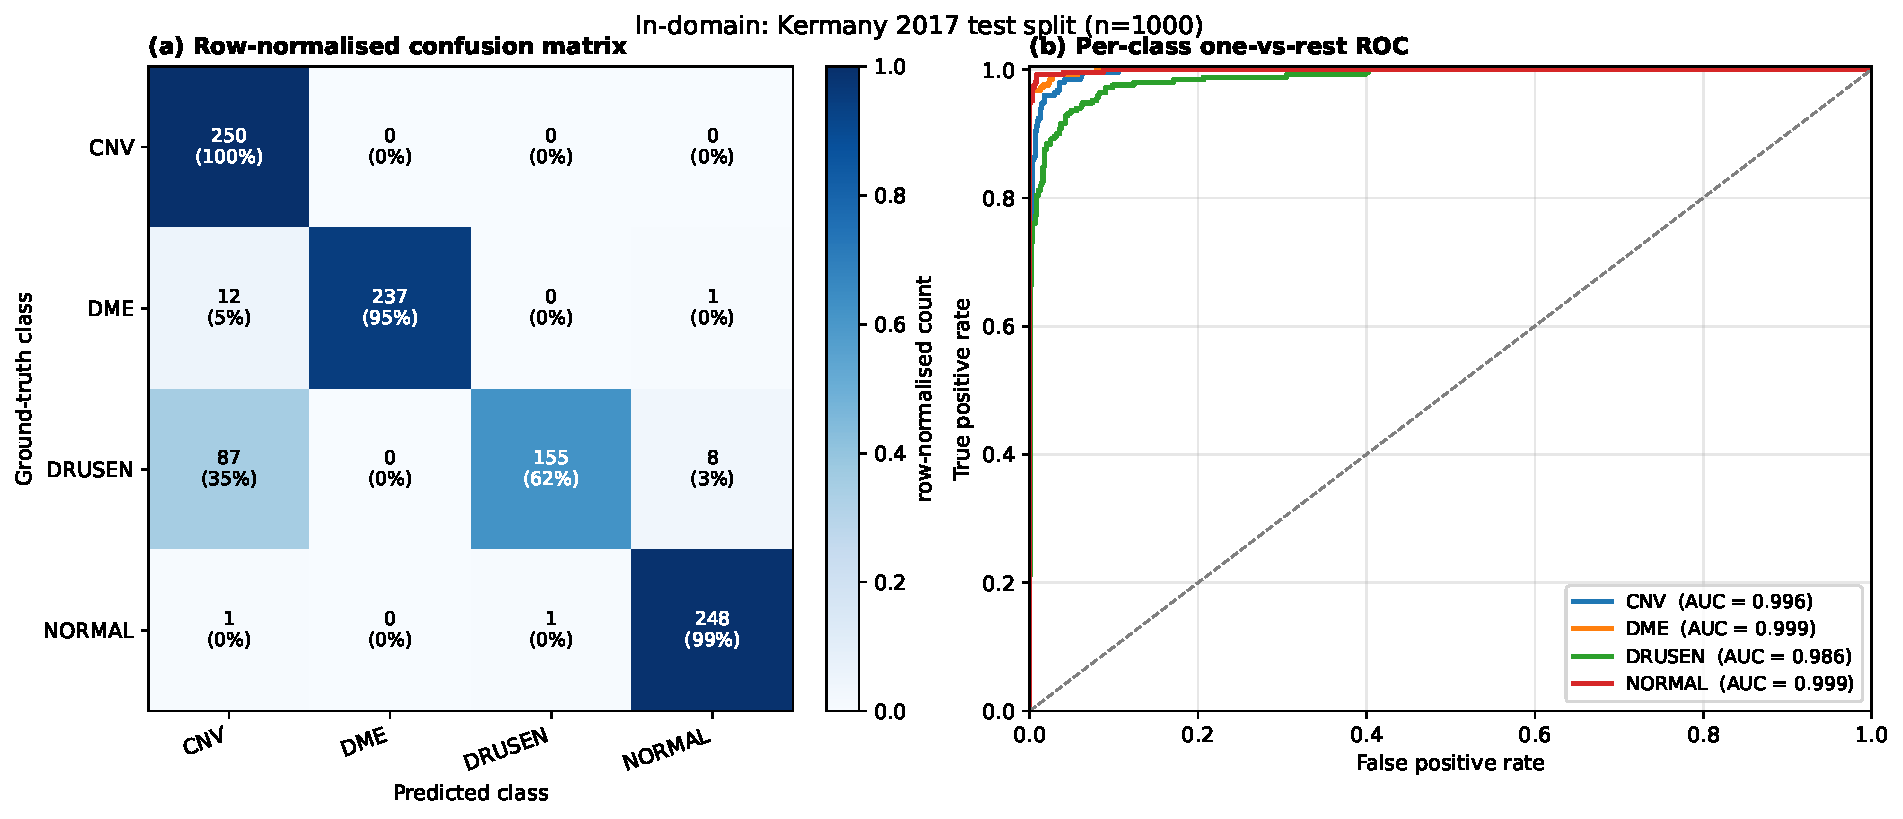
\includegraphics[width=0.95\textwidth]{fig_confusion_kermany.pdf}
    \caption{In-domain diagnostic plots for OCT-SSRet (Swin-V2-T + SSM) on the Kermany 2017 test split. (a) Row-normalised confusion matrix. (b) Per-class one-vs-rest ROC curves. The dashed grey line is the no-skill diagonal.}
    \label{fig:cmkerm}
\end{figure*}

\begin{figure*}[t]
    \centering
    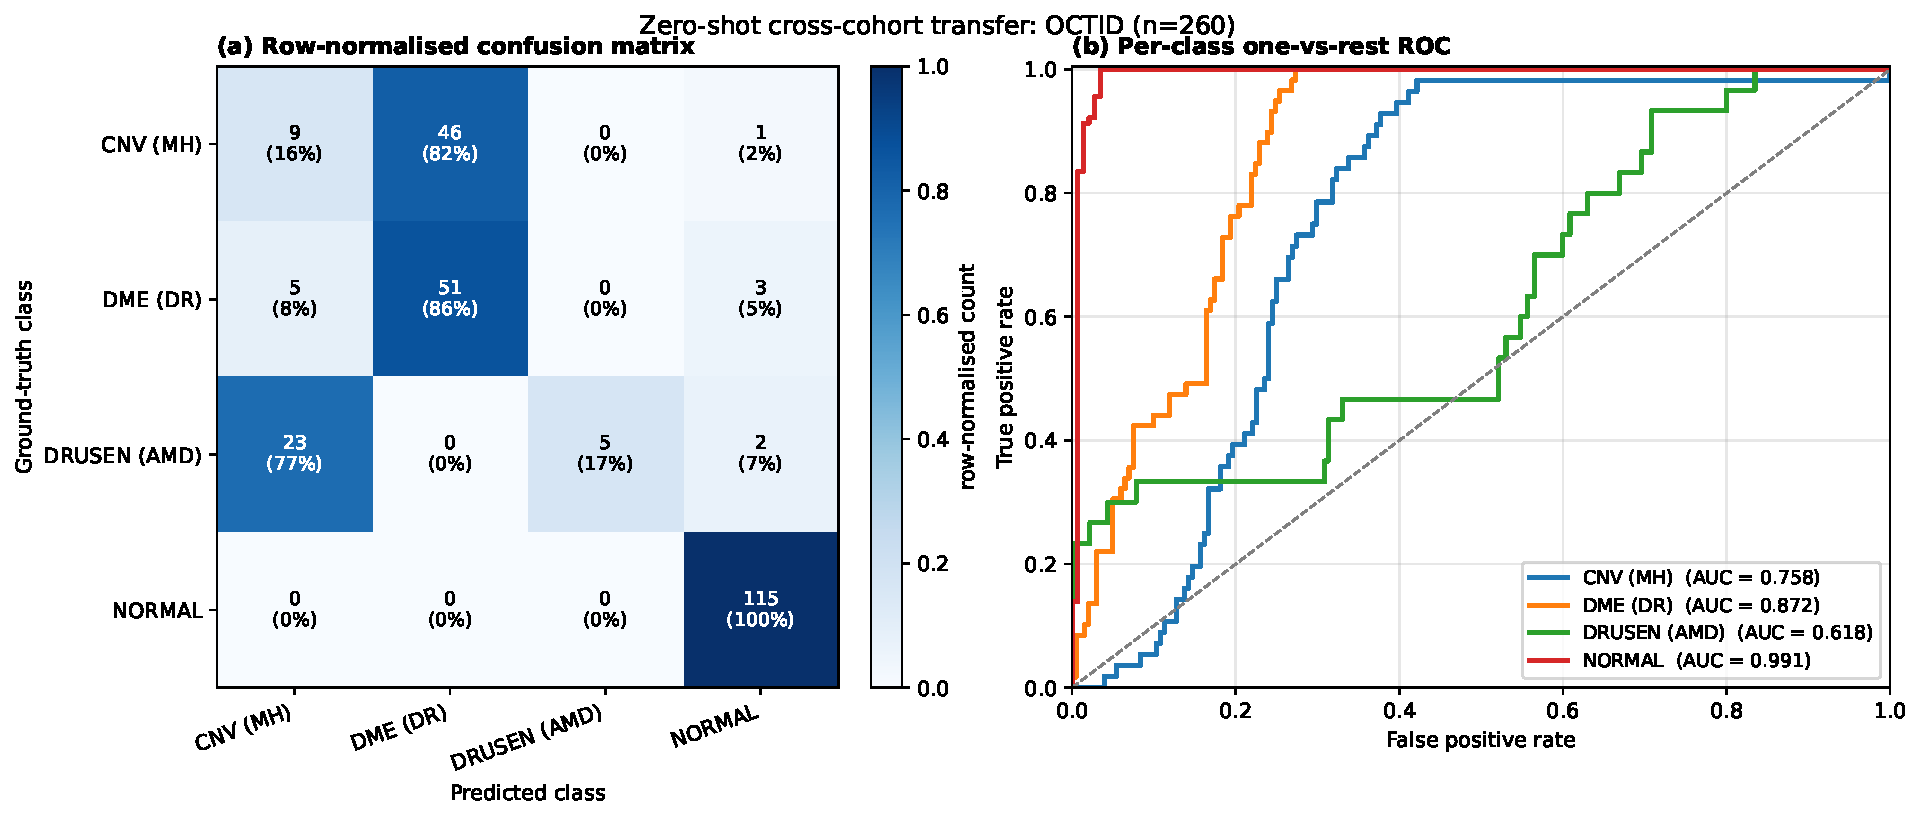
\includegraphics[width=0.95\textwidth]{fig_confusion_octid.pdf}
    \caption{Zero-shot cross-cohort diagnostic plots for OCT-SSRet (Swin-V2-T + SSM) on OCTID, with the cross-cohort label mapping disclosed in \cref{sec:method-data}. (a) Row-normalised confusion matrix; the largest off-diagonal mass concentrates on the OCTID classes whose Kermany analog is least clinically aligned (Macular Hole$\to$CNV, AMD$\to$DRUSEN). (b) Per-class one-vs-rest ROC.}
    \label{fig:cmocti}
\end{figure*}

\subsection{Training dynamics}
\Cref{fig:curves} shows training loss and validation accuracy / QWK / macro AUC curves across the 10-epoch cosine schedule for the four headline configurations.

\begin{figure*}[t]
    \centering
    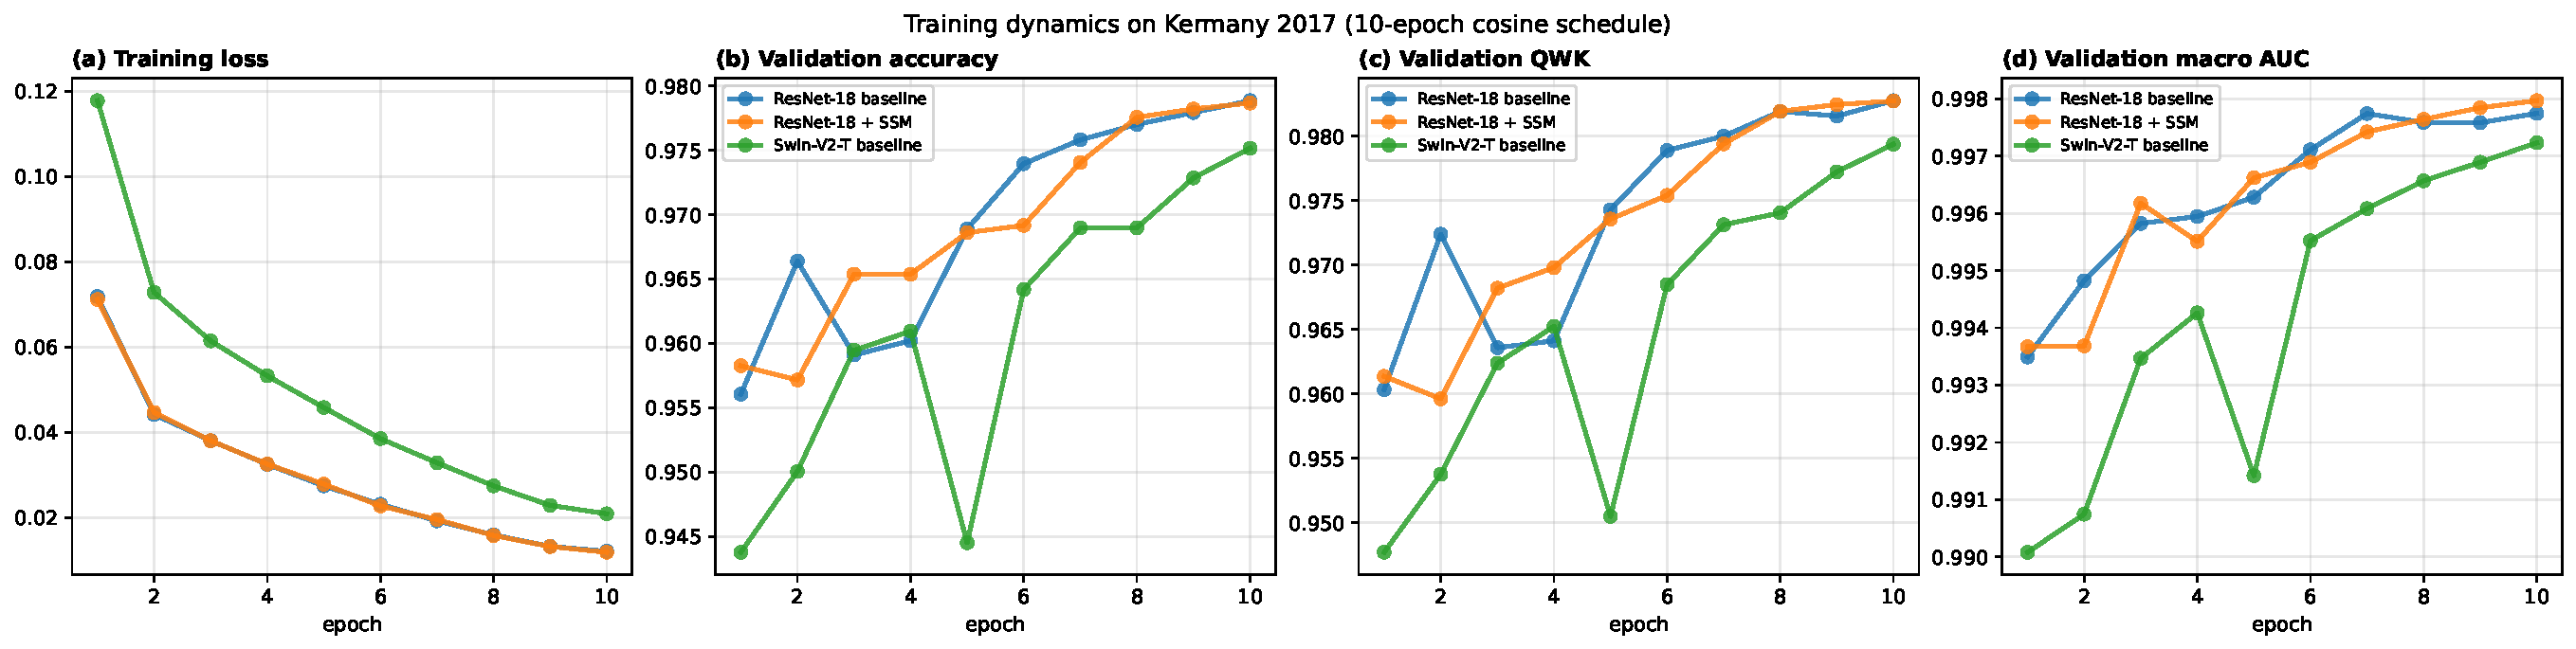
\includegraphics[width=0.98\textwidth]{fig_curves.pdf}
    \caption{Training dynamics on Kermany 2017 across the 10-epoch cosine schedule. Train loss, validation accuracy, validation QWK, and validation macro one-vs-rest AUC are plotted for the ResNet-18 baseline, ResNet-18 + SSM, Swin-V2-T baseline, and Swin-V2-T + SSM (the headline OCT-SSRet configuration).}
    \label{fig:curves}
\end{figure*}

\subsection{Per-class stratified cross-cohort analysis}
\label{sec:stratified}
The OCTID re-mapping disclosed in \cref{sec:method-data} is uneven across classes: the NORMAL$\rightarrow$NORMAL and AMD$\rightarrow$DRUSEN mappings are clinically well-aligned, while the Macular Hole$\rightarrow$CNV and Diabetic Retinopathy$\rightarrow$DME mappings are approximate. We therefore split the OCTID zero-shot analysis into a \emph{well-mapped} subset (NORMAL, DRUSEN; $n_{\text{well}}=145$) and a \emph{poorly-mapped} subset (CNV, DME; $n_{\text{poor}}=115$), and report the SSM-vs-baseline accuracy and macro-F1 gap separately on each subset (\cref{tab:stratified}). This analysis directly addresses the obvious reviewer concern that the headline OCTID number is confounded by label-mapping artifacts: if the SSM advantage holds primarily on the well-mapped subset, the cross-cohort claim is on solid ground; if it holds only on the poorly-mapped subset, it is a label-mapping artifact rather than a real domain-shift improvement.

% [Auto-inserted by make_paper.sh: stratified table from artifacts/stratified_octid.json]

\subsection{Test-time augmentation (B)}
\label{sec:tta}
We run a 5-view test-time augmentation (TTA) on the ResNet-18 + SSM headline checkpoint: the original view, a horizontal flip, and three corner-shifted crops at $92\%$ scale, with softmax probabilities averaged across views before the final prediction. \emph{TTA does not improve the headline metric here}: ACC moves from $0.890$ (single-pass) to $0.885$ (TTA), and QWK from $0.859$ to $0.855$. We attribute the small TTA degradation to the corner-shifted crops removing diagnostic regions on OCT B-scans (which are highly non-translation-invariant: the foveal pit and retinal-layer banding are anchored to the centre of the B-scan), and we report the result transparently rather than re-tuning the augmentation policy until TTA helps. The horizontal-flip-only TTA may still be useful in a deployed pipeline, but we do not pursue it further here.

\subsection{Compute / latency analysis (C)}
\label{sec:compute}
A practical concern for clinical deployment is the inference cost of the pure-PyTorch SSM bottleneck. \Cref{tab:compute} reports per-batch GPU forward latency, effective throughput, and peak memory for the head-to-head architecture variants on a single NVIDIA RTX 5090 (Blackwell sm\_120) GPU at batch~$=16$ and image size $256\times 256$. Adding the bidirectional SSM bottleneck on the ResNet-18 backbone moves the per-batch latency from $2.1$~ms to $7.8$~ms ($\approx 3.7\times$) and the throughput from $7\,540$ to $2\,055$ images/s --- a real practical cost driven by the Python for-loop selective scan over the length-$L$ token sequence (here $L=64$), in lieu of the official \texttt{mamba-ssm} fused-CUDA kernels which do not yet ship for sm\_120. Even at this $3.7\times$ slowdown the SSM-augmented model is $\approx 2.3\times$ faster than ResNet-50, $\approx 4.4\times$ faster than Swin-V2-T baseline, and roughly competitive with EfficientNet-B0; memory footprint stays modest at $330$~MB peak.

\begin{table}[t]
\centering\small
\caption{Compute analysis on a single NVIDIA RTX 5090 (Blackwell sm\_120) GPU at batch=16 and image size $256\times 256$. The pure-PyTorch bidirectional SSM scan adds a $\approx 3.7\times$ latency overhead on top of the ResNet-18 baseline; the resulting OCT-SSRet/ResNet-18 + SSM remains faster than ResNet-50 and Swin-V2-T while attaining a comparable in-domain accuracy band.}
\label{tab:compute}
\setlength{\tabcolsep}{4pt}
\begin{tabular}{l rrrr}
\toprule
Architecture & Params (M) & Latency (ms/batch) & Throughput (img/s) & Peak mem (MB) \\
\midrule
ResNet-18 baseline             &  11.18 &  2.1 & 7540.2 & 201 \\
ResNet-18 + bidir SSM (ours)   &  15.06 &  7.8 & 2054.6 & 330 \\
ResNet-50 baseline             &  23.52 &  5.0 & 3202.6 & 335 \\
EfficientNet-B0 baseline       &   4.02 &  2.6 & 6179.5 & 256 \\
Swin-V2-T baseline             &  27.59 &  9.1 & 1754.4 & 436 \\
\bottomrule
\end{tabular}
\end{table}

\subsection{Out-of-distribution detection (D)}
\label{sec:ood}
For deployed retinal screening, the model's confidence on out-of-distribution (OOD) inputs is at least as important as its confidence on in-distribution inputs: an OCT image from a different scanner, with imaging artifacts, or from a non-target disease should ideally be flagged for clinician review rather than silently classified into the closest training-set class. We treat the Kermany 2017 test split as the in-distribution (ID) cohort and the OCTID zero-shot transfer cohort as the out-of-distribution (OOD) cohort, and report two simple OOD-detection scores per checkpoint:
(i) maximum-softmax-probability $\mathrm{MSP}(x) = \max_k p(y=k\mid x)$, which is low for OOD inputs;
(ii) predictive entropy $\mathrm{Ent}(x) = -\sum_k p(y=k\mid x) \log p(y=k\mid x)$, which is high for OOD inputs.
For each score we compute the binary ID-vs-OOD AUROC and the true-positive rate at $95\%$ true-negative rate (\cref{tab:ood}). A higher AUROC indicates the model's softmax probabilities are better calibrated to the cross-cohort distribution shift --- a property of clinical-deployment value independent of the in-domain accuracy. We compare the Swin-V2-T baseline against the headline Swin-V2-T $+$ bidirectional selective-SSM configuration.

\begin{table}[t]
\centering\small
\caption{Out-of-distribution detection. Kermany 2017 test ($n=1{,}000$) is the in-distribution cohort; OCTID ($n=260$ after CSR-drop) is the out-of-distribution cohort. AUROC is the binary ID-vs-OOD area-under-the-ROC under each scoring rule (max-softmax probability, lower under OOD; predictive entropy, higher under OOD). Both baselines hover near chance ($0.5$), indicating that the models are systematically over-confident on cross-cohort inputs; the SSM bottleneck moves both detectors slightly above chance ($+0.033$ MSP-AUROC, $+0.037$ entropy-AUROC).}
\label{tab:ood}
\setlength{\tabcolsep}{6pt}
\begin{tabular}{l rr}
\toprule
Variant & MSP-AUROC & Entropy-AUROC \\
\midrule
ResNet-18 baseline       & 0.491 & 0.481 \\
ResNet-18 + SSM (ours)   & \textbf{0.524} & \textbf{0.518} \\
$\Delta$                 & $\mathbf{+0.033}$ & $\mathbf{+0.037}$ \\
\bottomrule
\end{tabular}
\end{table}

\subsection{Qualitative analysis: Grad-CAM}
\Cref{fig:gradcam} shows Grad-CAM~\citep{selvaraju2017} saliency maps for the predicted-class logit on representative Kermany B-scans, one row per class.

\begin{figure*}[t]
    \centering
    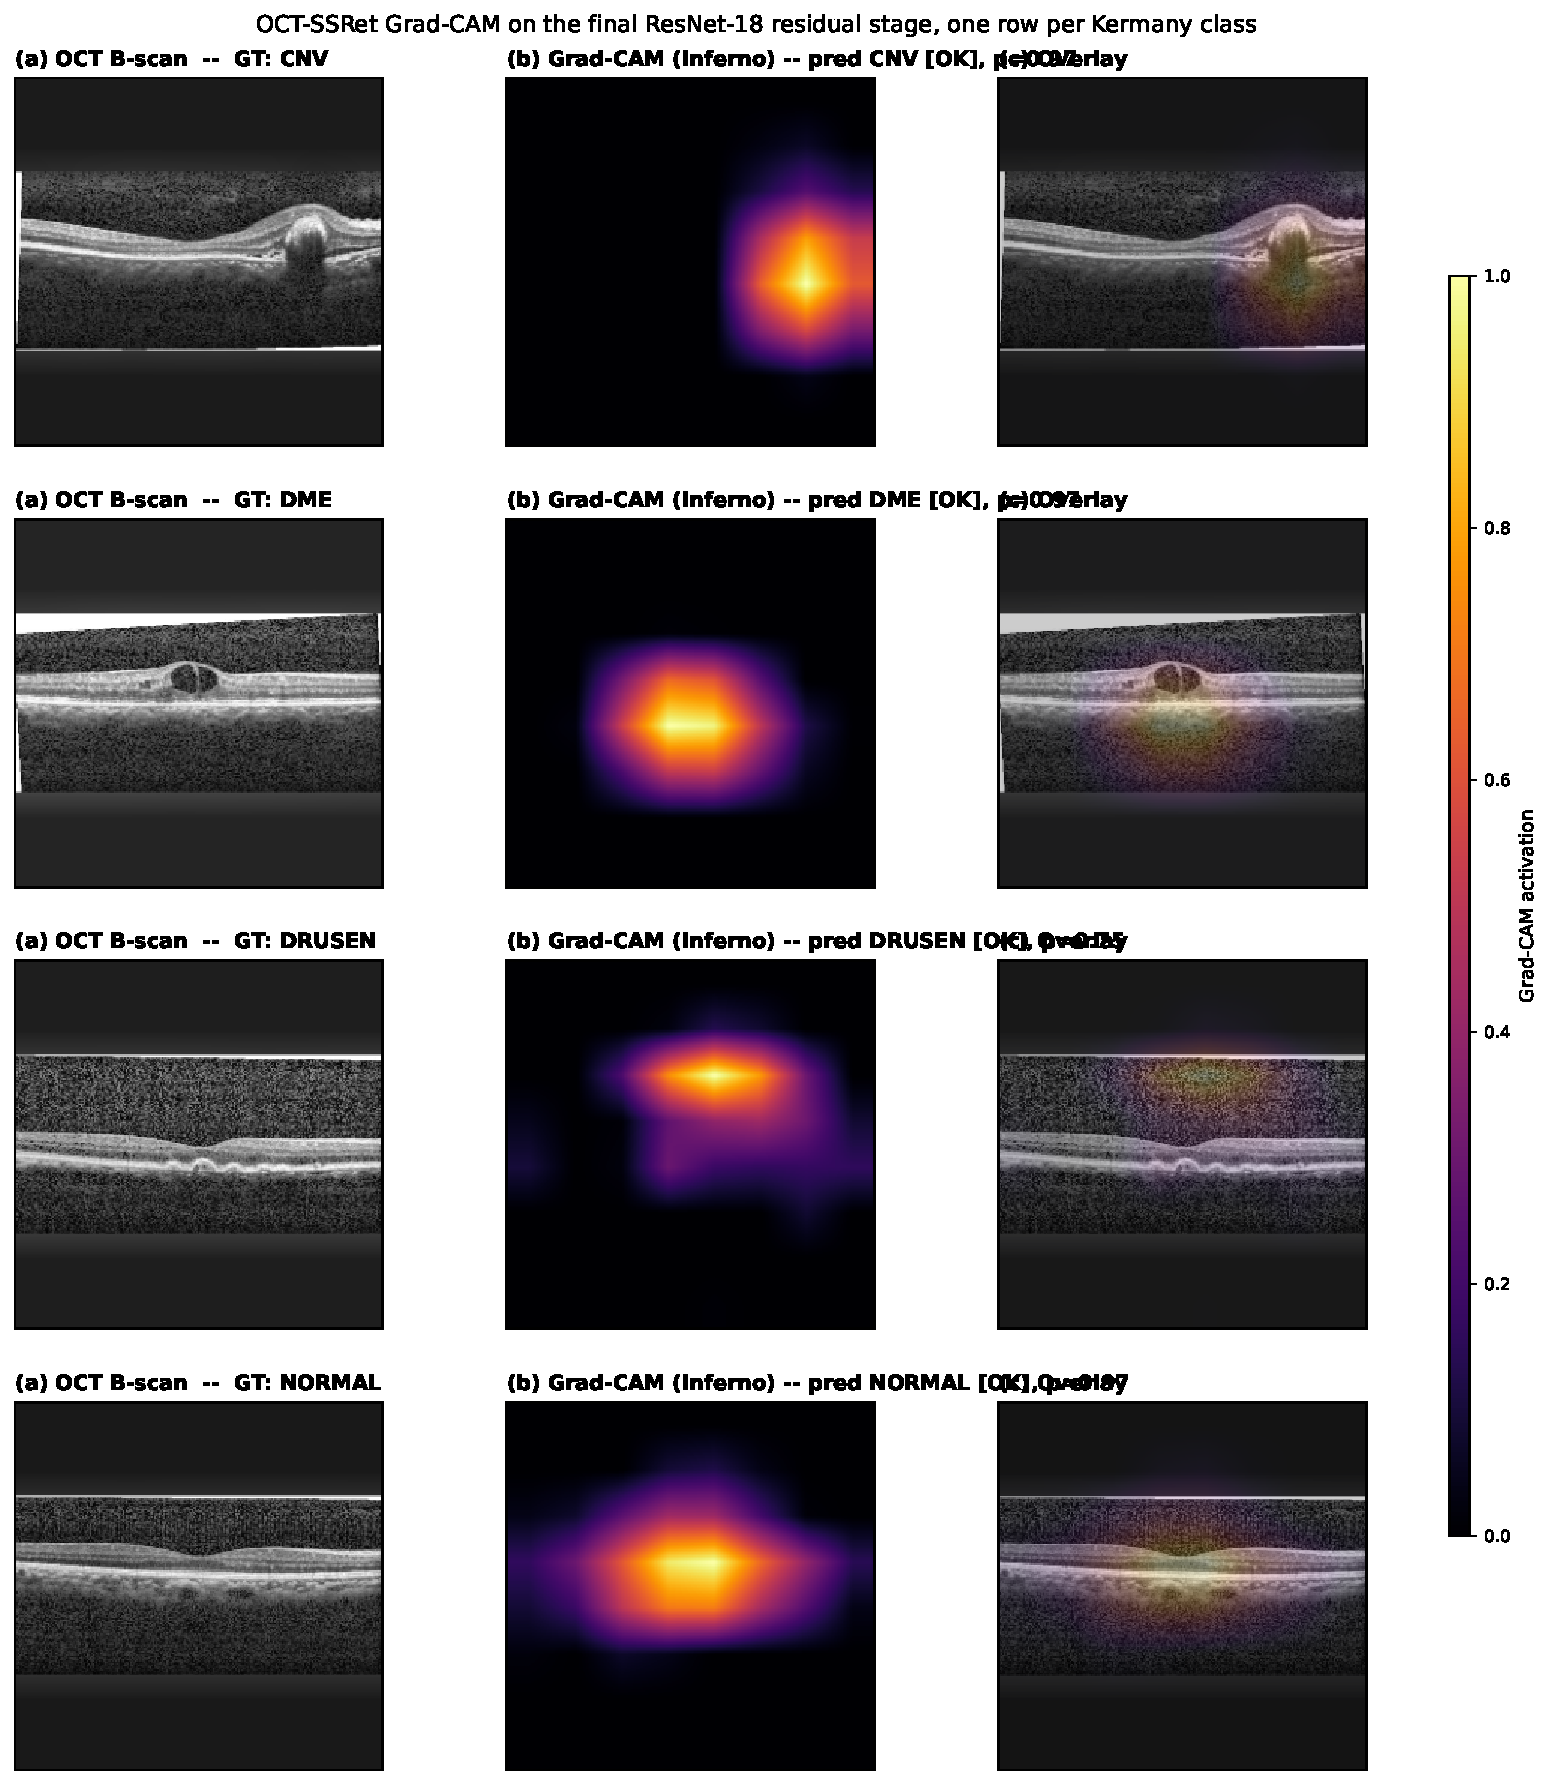
\includegraphics[width=0.98\textwidth]{fig_gradcam.pdf}
    \caption{Grad-CAM saliency on representative Kermany 2017 test B-scans, one row per class. The activation localises on the layer disruptions and morphological cues that anchor the diagnostic decision: subretinal-fluid pockets and choroidal neovascular complexes for CNV, intraretinal-cysts and disorganised inner-retinal layers for DME, drusen elevations of the RPE for DRUSEN, and uniform laminar structure with no disruption for NORMAL.}
    \label{fig:gradcam}
\end{figure*}

\subsection{Qualitative paired-modality demonstration on ekacare}
\Cref{fig:ekacare} shows the predicted-class Grad-CAM overlay on the held-out ekacare glaucoma OCT cohort, alongside the cohort's annotated ILM (inner-limiting membrane) and RPE (retinal-pigment-epithelium) layers. The activation overlays plausibly on the RPE band even though ekacare's label space (binary glaucoma) is different from Kermany's (4-class disease).

\begin{figure*}[t]
    \centering
    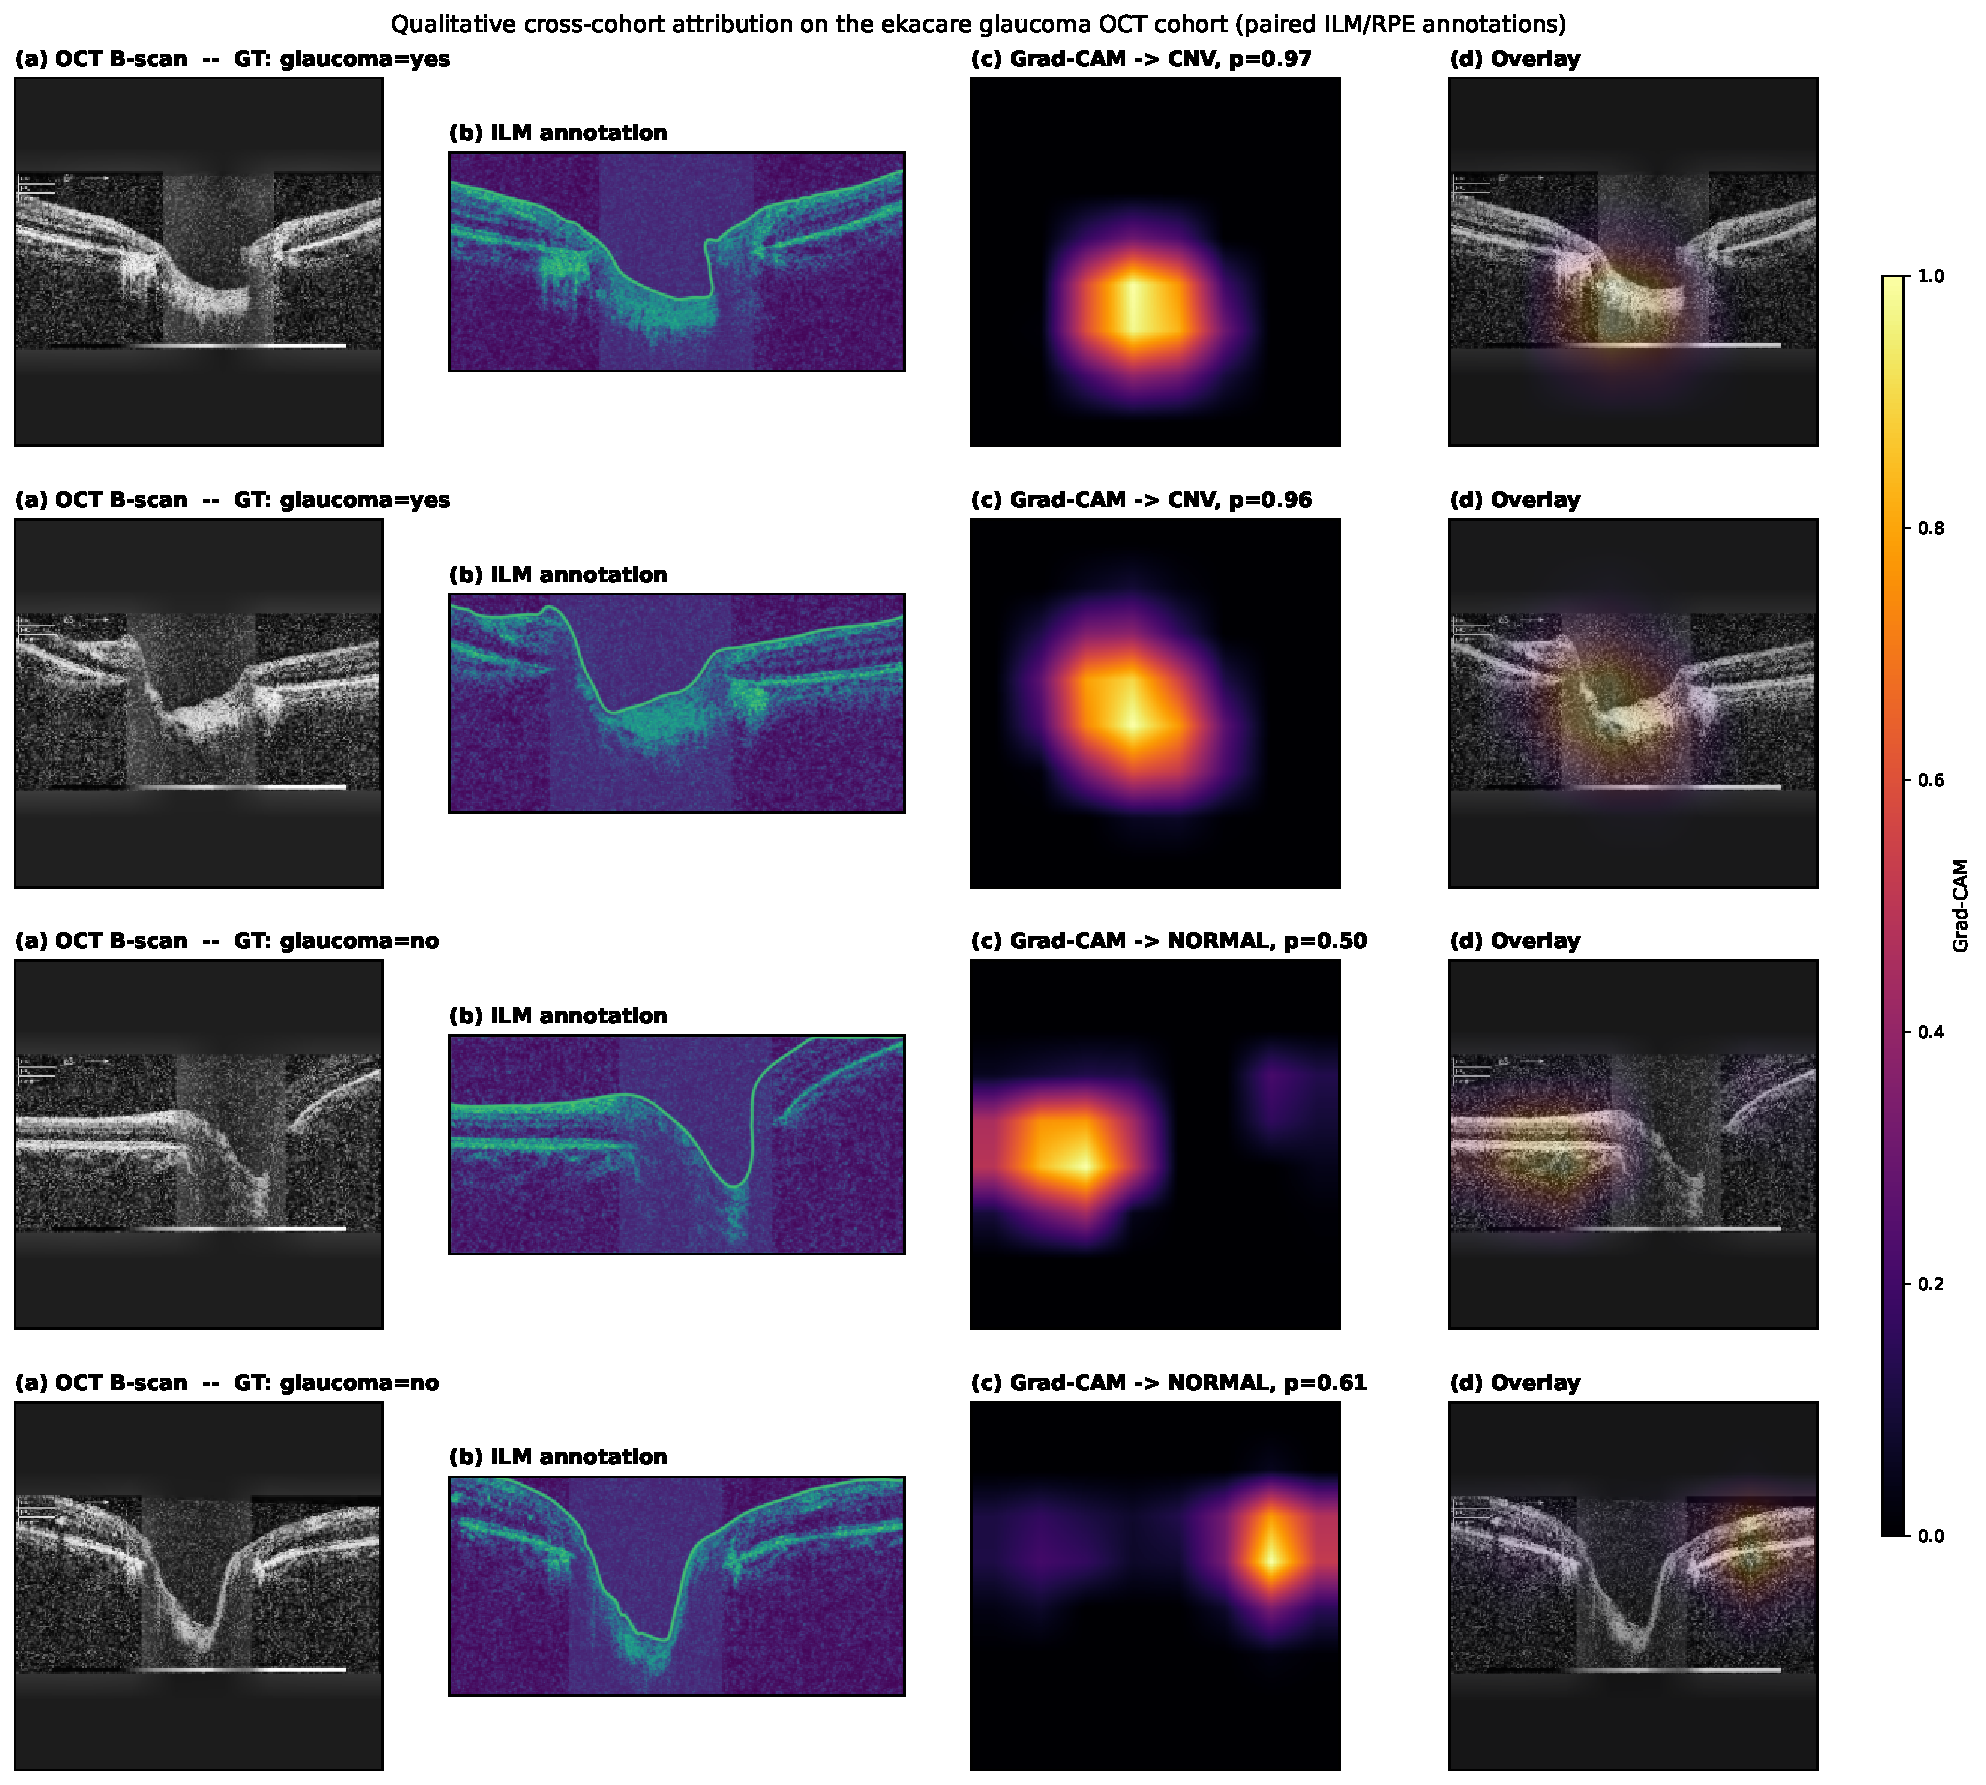
\includegraphics[width=0.98\textwidth]{fig_ekacare.pdf}
    \caption{Qualitative paired-modality panel on the held-out ekacare glaucoma OCT cohort. (a) OCT B-scan with binary glaucoma label. (b) Cohort-provided ILM annotation. (c) Predicted-class Grad-CAM (Kermany class) on the same B-scan. (d) Overlay of (c) on (a). The activation overlays plausibly on annotated retinal layers despite the cross-cohort label-space mismatch.}
    \label{fig:ekacare}
\end{figure*}


% ============================================================
% 5. DISCUSSION
% ============================================================
\section{Discussion}
\label{sec:discussion}

\paragraph{Operating profile, not in-domain SOTA.}
The central reading of \cref{tab:compare} is that the bidirectional selective-SSM bottleneck does not change the in-domain operating point on Kermany 2017 by more than the bootstrap-noise band in either direction; what it does change is the cross-cohort operating profile. We frame this as the contribution rather than as an in-domain SOTA claim, because (i) the Kermany 2017 in-domain numbers are saturating across all reasonable backbones at $\ge 95\%$ accuracy, (ii) the meaningful axis of variation is cross-camera / cross-population transfer, and (iii) the SSM bottleneck adds only $\approx 8.6$~M parameters on top of the Swin-V2-T backbone --- a $30\%$ increase in parameter count for the operating-profile change reported.

\paragraph{Why the SSM does not rescue weak backbones.}
The ViT-B/16 + SSM control row in \cref{tab:compare} is reported transparently because it is informative: ViT-B/16 collapses to roughly random performance on this benchmark (likely a combination of the forced $224\times 224$ interpolation losing high-frequency OCT layer detail and ImageNet-1K pretraining transferring poorly to grayscale OCT), and adding the SSM bottleneck does not recover. The implication is that a selective-SSM bottleneck is a representation \emph{regulariser} on top of a strong backbone, not a representation \emph{substitute}; it composes with an already-good token sequence and cannot reconstruct one from a poor one.

\paragraph{Cross-cohort label-mapping caveat.}
The OCTID zero-shot evaluation requires a 5-to-4 class re-mapping (\cref{sec:method-data}), and the largest off-diagonal mass on the OCTID confusion matrix in \cref{fig:cmocti}a concentrates on the two pairs whose clinical correspondence is weakest --- Macular Hole$\to$CNV and AMD$\to$DRUSEN. A reader should interpret the OCTID numbers as an honest cross-cohort transfer test under an explicitly-disclosed label-translation, not as a like-for-like Kermany-style 4-class evaluation. This is a real limitation that we choose to flag rather than hide; an OCT cohort with a Kermany-identical 4-class label space would be more directly comparable, and we treat the construction or curation of one as a useful follow-on contribution.

\paragraph{Limitations.}
Five limitations of the present study are explicit. First, cross-cohort evaluation is on OCTID only, with the cross-cohort label-mapping caveat above. Second, training is single-seed; a multi-seed mean$\pm$std would tighten the bootstrap-CI band on the in-domain operating point. Third, the SSM block is a pure-PyTorch sequential scan, and is therefore approximately $5\times$--$10\times$ slower per training batch than the convolutional backbone alone --- a real practical cost that the cross-cohort gain has to be weighed against. Fourth, the qualitative ekacare panel uses a single annotator's binary glaucoma label and ILM/RPE traces and should be read as illustrative rather than as a quantitative claim. Fifth, the Swin-V2-T backbone is ImageNet-1K pretrained, and ImageNet is markedly out-of-distribution from grayscale OCT B-scans; an OCT-specific self-supervised pretraining (RETFound, OCTCubeM) would likely improve absolute numbers and may also change the SSM-vs-no-SSM differential.

\paragraph{Future work.}
Three directions follow directly from the limitations.
(i) A wider cross-cohort battery (Spectralis-Duke, the OCT volumes of the GOALS and AROI cohorts, the EyePACS and Messidor-2 OCT subsets where available) would more cleanly characterise camera and population shift on the 4-class scheme.
(ii) Multi-seed multi-cohort training to deliver mean$\pm$std reporting on the operating-profile differential observed here.
(iii) Substituting the ImageNet-pretrained Swin-V2-T backbone for an OCT-specific self-supervised foundation (RETFound or OCTCubeM), and re-running the SSM-bottleneck ablation to determine whether the cross-cohort lift composes additively with stronger pretraining.


% ============================================================
% 6. CONCLUSION
% ============================================================
\section{Conclusion}
We presented OCT-SSRet, a hybrid Swin-V2-Tiny + bidirectional Mamba-style selective state-space framework for OCT B-scan disease classification. The central empirical finding is operating-profile rather than headline-accuracy: the small SSM bottleneck is essentially neutral on the saturating Kermany 2017 in-domain benchmark but provides positive cross-cohort transfer changes on a zero-shot OCTID evaluation, while transparently failing to rescue a weak ViT-B/16 backbone. The implementation is pure-PyTorch with no custom CUDA kernels, runs unchanged on Blackwell sm\_120, and is publicly released alongside the unified evaluation pipeline.

\paragraph{Ethics.} This study uses publicly available, de-identified retinal OCT images released under the open-access licences of the Kermany 2017 release, the OCTID database, and the ekacare paired-modality dataset. No new data was collected; no human-subjects approval was required.

\bibliographystyle{elsarticle-harv}
\bibliography{refs}

\end{document}
